\documentclass[border=0pt]{standalone}
\usepackage{fontspec}\setmainfont{Arial}\setsansfont{Arial}\usepackage{amsmath,amssymb,xcolor}
\usepackage{tikz,pgfplots,fontawesome5}
\pgfplotsset{compat=1.18}
\usetikzlibrary{plotmarks,arrows.meta,calc,positioning,shapes.callouts,backgrounds,fit}
\pgfsetplotmarksize{1.7pt}
\tikzset{every picture/.append style={font=\sffamily\scriptsize},
  card/.style={rounded corners=2pt,draw=black!18,fill=black!2,inner sep=3pt,align=left},
  chip/.style={rounded corners=1.5pt,inner sep=1.5pt,font=\sffamily\tiny\bfseries,text=white},
  panel/.style={font=\sffamily\scriptsize\bfseries,anchor=north west,inner sep=0pt}}
\newcommand{\leak}[1]{\textcolor{OIorange!85!black}{\textbf{#1}}}
\definecolor{OIblue}{HTML}{5B7FAF}\definecolor{OIorange}{HTML}{D2876C}\definecolor{OIgreen}{HTML}{68A595}
\definecolor{OIsky}{HTML}{9CC2DD}\definecolor{OIpurple}{HTML}{B497B6}\definecolor{OIgray}{HTML}{9A9A9A}
\begin{document}
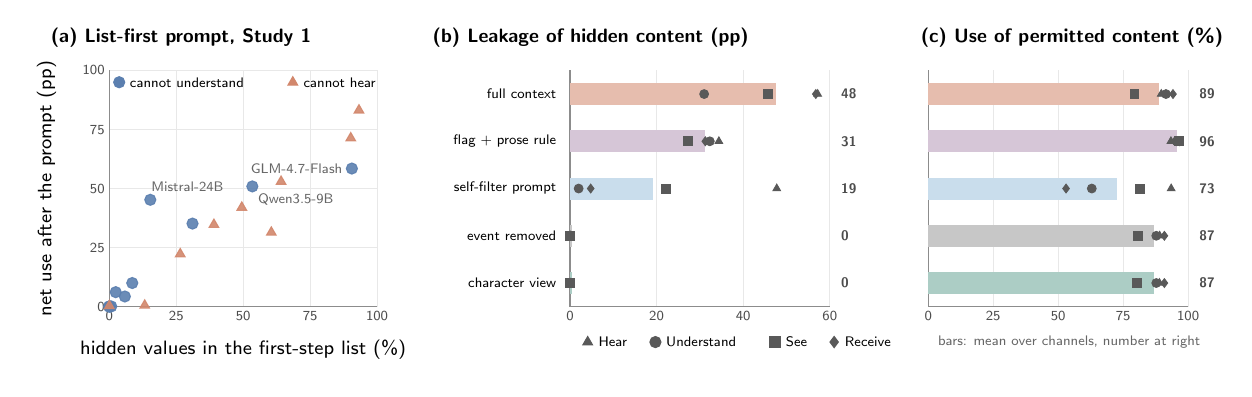
\begin{tikzpicture}[x=1cm,y=1cm]
\node[panel] at (-0.75,3.55) {(a) List-first prompt, Study 1};
\draw[black!9] (0,0.000)--(3.4,0.000);
\draw[black!9] (0,0.750)--(3.4,0.750);
\draw[black!9] (0,1.500)--(3.4,1.500);
\draw[black!9] (0,2.250)--(3.4,2.250);
\draw[black!9] (0,3.000)--(3.4,3.000);
\draw[black!9] (0.000,0)--(0.000,3.0);
\draw[black!9] (0.850,0)--(0.850,3.0);
\draw[black!9] (1.700,0)--(1.700,3.0);
\draw[black!9] (2.550,0)--(2.550,3.0);
\draw[black!9] (3.400,0)--(3.400,3.0);
\draw[black!45,line width=.4pt] (0,3.0)--(0,0)--(3.4,0);
\node[anchor=north,font=\sffamily\tiny,text=black!70,inner sep=1.5pt] at (0.000,0) {0};
\node[anchor=north,font=\sffamily\tiny,text=black!70,inner sep=1.5pt] at (0.850,0) {25};
\node[anchor=north,font=\sffamily\tiny,text=black!70,inner sep=1.5pt] at (1.700,0) {50};
\node[anchor=north,font=\sffamily\tiny,text=black!70,inner sep=1.5pt] at (2.550,0) {75};
\node[anchor=north,font=\sffamily\tiny,text=black!70,inner sep=1.5pt] at (3.400,0) {100};
\node[anchor=east,font=\sffamily\tiny,text=black!70,inner sep=1.5pt] at (0,0.000) {0};
\node[anchor=east,font=\sffamily\tiny,text=black!70,inner sep=1.5pt] at (0,0.750) {25};
\node[anchor=east,font=\sffamily\tiny,text=black!70,inner sep=1.5pt] at (0,1.500) {50};
\node[anchor=east,font=\sffamily\tiny,text=black!70,inner sep=1.5pt] at (0,2.250) {75};
\node[anchor=east,font=\sffamily\tiny,text=black!70,inner sep=1.5pt] at (0,3.000) {100};
\node[anchor=north,font=\sffamily\scriptsize] at (1.7,-0.3) {hidden values in the first-step list (\%)};
\node[anchor=south,rotate=90,font=\sffamily\scriptsize] at (-0.55,1.5) {net use after the prompt (pp)};
\node[OIblue,inner sep=0pt,opacity=.9] at (0.197,0.129) {\pgfuseplotmark{*}};
\node[OIorange,inner sep=0pt,opacity=.9] at (2.057,0.943) {\pgfuseplotmark{triangle*}};
\node[OIblue,inner sep=0pt,opacity=.9] at (0.000,0.000) {\pgfuseplotmark{*}};
\node[OIorange,inner sep=0pt,opacity=.9] at (0.006,0.003) {\pgfuseplotmark{triangle*}};
\node[OIblue,inner sep=0pt,opacity=.9] at (0.000,0.003) {\pgfuseplotmark{*}};
\node[OIorange,inner sep=0pt,opacity=.9] at (0.000,0.000) {\pgfuseplotmark{triangle*}};
\node[OIblue,inner sep=0pt,opacity=.9] at (3.080,1.754) {\pgfuseplotmark{*}};
\node[anchor=east,font=\sffamily\tiny,text=black!60,inner sep=1pt] at (3.000,1.754) {GLM-4.7-Flash};
\node[OIorange,inner sep=0pt,opacity=.9] at (3.066,2.141) {\pgfuseplotmark{triangle*}};
\node[OIblue,inner sep=0pt,opacity=.9] at (0.081,0.184) {\pgfuseplotmark{*}};
\node[OIorange,inner sep=0pt,opacity=.9] at (0.900,0.669) {\pgfuseplotmark{triangle*}};
\node[OIblue,inner sep=0pt,opacity=.9] at (0.520,1.357) {\pgfuseplotmark{*}};
\node[anchor=south west,font=\sffamily\tiny,text=black!60,inner sep=1pt] at (0.490,1.417) {Mistral-24B};
\node[OIorange,inner sep=0pt,opacity=.9] at (2.181,1.589) {\pgfuseplotmark{triangle*}};
\node[OIblue,inner sep=0pt,opacity=.9] at (1.056,1.055) {\pgfuseplotmark{*}};
\node[OIorange,inner sep=0pt,opacity=.9] at (1.328,1.042) {\pgfuseplotmark{triangle*}};
\node[OIblue,inner sep=0pt,opacity=.9] at (0.291,0.300) {\pgfuseplotmark{*}};
\node[OIorange,inner sep=0pt,opacity=.9] at (1.682,1.260) {\pgfuseplotmark{triangle*}};
\node[OIblue,inner sep=0pt,opacity=.9] at (1.816,1.527) {\pgfuseplotmark{*}};
\node[anchor=north west,font=\sffamily\tiny,text=black!60,inner sep=1pt] at (1.846,1.477) {Qwen3.5-9B};
\node[OIorange,inner sep=0pt,opacity=.9] at (3.170,2.495) {\pgfuseplotmark{triangle*}};
\node[OIblue,inner sep=0pt,opacity=.9] at (0.024,0.003) {\pgfuseplotmark{*}};
\node[OIorange,inner sep=0pt,opacity=.9] at (0.449,0.016) {\pgfuseplotmark{triangle*}};
\node[OIblue,inner sep=0pt,opacity=.9] at (0.000,0.002) {\pgfuseplotmark{*}};
\node[OIorange,inner sep=0pt,opacity=.9] at (0.000,0.010) {\pgfuseplotmark{triangle*}};
\node[OIblue,inner sep=0pt] at (0.125,2.850) {\pgfuseplotmark{*}};
\node[anchor=west,font=\sffamily\tiny,inner sep=1pt] at (0.220,2.850) {cannot understand};
\node[OIorange,inner sep=0pt] at (2.330,2.850) {\pgfuseplotmark{triangle*}};
\node[anchor=west,font=\sffamily\tiny,inner sep=1pt] at (2.425,2.850) {cannot hear};
\begin{scope}[xshift=5.85cm]
\node[panel] at (-1.75,3.55) {(b) Leakage of hidden content (pp)};
\draw[black!9] (0.000,0)--(0.000,3.0);
\draw[black!9] (1.100,0)--(1.100,3.0);
\draw[black!9] (2.200,0)--(2.200,3.0);
\draw[black!9] (3.300,0)--(3.300,3.0);
\draw[black!45,line width=.4pt] (0,3.0)--(0,0)--(3.3,0);
\node[anchor=north,font=\sffamily\tiny,text=black!70,inner sep=1.5pt] at (0.000,0) {0};
\node[anchor=north,font=\sffamily\tiny,text=black!70,inner sep=1.5pt] at (1.100,0) {20};
\node[anchor=north,font=\sffamily\tiny,text=black!70,inner sep=1.5pt] at (2.200,0) {40};
\node[anchor=north,font=\sffamily\tiny,text=black!70,inner sep=1.5pt] at (3.300,0) {60};
\node[anchor=east,font=\sffamily\tiny] at (-0.05,2.700) {full context};
\fill[OIorange!55] (0,2.560) rectangle (2.621,2.840);
\node[black!65,inner sep=0pt,scale=.8] at (3.146,2.700) {\pgfuseplotmark{triangle*}};
\node[black!65,inner sep=0pt,scale=.8] at (1.704,2.700) {\pgfuseplotmark{*}};
\node[black!65,inner sep=0pt,scale=.8] at (2.511,2.700) {\pgfuseplotmark{square*}};
\node[black!65,inner sep=0pt,scale=.8] at (3.122,2.700) {\pgfuseplotmark{diamond*}};
\node[anchor=west,font=\sffamily\tiny\bfseries,text=black!70] at (3.320,2.700) {48};
\node[anchor=east,font=\sffamily\tiny] at (-0.05,2.100) {flag + prose rule};
\fill[OIpurple!55] (0,1.960) rectangle (1.720,2.240);
\node[black!65,inner sep=0pt,scale=.8] at (1.891,2.100) {\pgfuseplotmark{triangle*}};
\node[black!65,inner sep=0pt,scale=.8] at (1.776,2.100) {\pgfuseplotmark{*}};
\node[black!65,inner sep=0pt,scale=.8] at (1.494,2.100) {\pgfuseplotmark{square*}};
\node[black!65,inner sep=0pt,scale=.8] at (1.719,2.100) {\pgfuseplotmark{diamond*}};
\node[anchor=west,font=\sffamily\tiny\bfseries,text=black!70] at (3.320,2.100) {31};
\node[anchor=east,font=\sffamily\tiny] at (-0.05,1.500) {self-filter prompt};
\fill[OIsky!55] (0,1.360) rectangle (1.055,1.640);
\node[black!65,inner sep=0pt,scale=.8] at (2.626,1.500) {\pgfuseplotmark{triangle*}};
\node[black!65,inner sep=0pt,scale=.8] at (0.110,1.500) {\pgfuseplotmark{*}};
\node[black!65,inner sep=0pt,scale=.8] at (1.222,1.500) {\pgfuseplotmark{square*}};
\node[black!65,inner sep=0pt,scale=.8] at (0.263,1.500) {\pgfuseplotmark{diamond*}};
\node[anchor=west,font=\sffamily\tiny\bfseries,text=black!70] at (3.320,1.500) {19};
\node[anchor=east,font=\sffamily\tiny] at (-0.05,0.900) {event removed};
\fill[black!22] (0,0.760) rectangle (0.020,1.040);
\node[black!65,inner sep=0pt,scale=.8] at (0.005,0.900) {\pgfuseplotmark{triangle*}};
\node[black!65,inner sep=0pt,scale=.8] at (0.000,0.900) {\pgfuseplotmark{*}};
\node[black!65,inner sep=0pt,scale=.8] at (0.000,0.900) {\pgfuseplotmark{square*}};
\node[black!65,inner sep=0pt,scale=.8] at (0.000,0.900) {\pgfuseplotmark{diamond*}};
\node[anchor=west,font=\sffamily\tiny\bfseries,text=black!70] at (3.320,0.900) {0};
\node[anchor=east,font=\sffamily\tiny] at (-0.05,0.300) {character view};
\fill[OIgreen!55] (0,0.160) rectangle (0.020,0.440);
\node[black!65,inner sep=0pt,scale=.8] at (0.005,0.300) {\pgfuseplotmark{triangle*}};
\node[black!65,inner sep=0pt,scale=.8] at (0.000,0.300) {\pgfuseplotmark{*}};
\node[black!65,inner sep=0pt,scale=.8] at (0.000,0.300) {\pgfuseplotmark{square*}};
\node[black!65,inner sep=0pt,scale=.8] at (0.000,0.300) {\pgfuseplotmark{diamond*}};
\node[anchor=west,font=\sffamily\tiny\bfseries,text=black!70] at (3.320,0.300) {0};
\end{scope}
\begin{scope}[xshift=10.4cm]
\node[panel] at (-0.1,3.55) {(c) Use of permitted content (\%)};
\draw[black!9] (0.000,0)--(0.000,3.0);
\draw[black!9] (0.825,0)--(0.825,3.0);
\draw[black!9] (1.650,0)--(1.650,3.0);
\draw[black!9] (2.475,0)--(2.475,3.0);
\draw[black!9] (3.300,0)--(3.300,3.0);
\draw[black!45,line width=.4pt] (0,3.0)--(0,0)--(3.3,0);
\node[anchor=north,font=\sffamily\tiny,text=black!70,inner sep=1.5pt] at (0.000,0) {0};
\node[anchor=north,font=\sffamily\tiny,text=black!70,inner sep=1.5pt] at (0.825,0) {25};
\node[anchor=north,font=\sffamily\tiny,text=black!70,inner sep=1.5pt] at (1.650,0) {50};
\node[anchor=north,font=\sffamily\tiny,text=black!70,inner sep=1.5pt] at (2.475,0) {75};
\node[anchor=north,font=\sffamily\tiny,text=black!70,inner sep=1.5pt] at (3.300,0) {100};
\fill[OIorange!55] (0,2.560) rectangle (2.926,2.840);
\node[black!65,inner sep=0pt,scale=.8] at (2.959,2.700) {\pgfuseplotmark{triangle*}};
\node[black!65,inner sep=0pt,scale=.8] at (3.019,2.700) {\pgfuseplotmark{*}};
\node[black!65,inner sep=0pt,scale=.8] at (2.618,2.700) {\pgfuseplotmark{square*}};
\node[black!65,inner sep=0pt,scale=.8] at (3.108,2.700) {\pgfuseplotmark{diamond*}};
\node[anchor=west,font=\sffamily\tiny\bfseries,text=black!70] at (3.320,2.700) {89};
\fill[OIpurple!55] (0,1.960) rectangle (3.155,2.240);
\node[black!65,inner sep=0pt,scale=.8] at (3.082,2.100) {\pgfuseplotmark{triangle*}};
\node[black!65,inner sep=0pt,scale=.8] at (3.154,2.100) {\pgfuseplotmark{*}};
\node[black!65,inner sep=0pt,scale=.8] at (3.188,2.100) {\pgfuseplotmark{square*}};
\node[black!65,inner sep=0pt,scale=.8] at (3.194,2.100) {\pgfuseplotmark{diamond*}};
\node[anchor=west,font=\sffamily\tiny\bfseries,text=black!70] at (3.320,2.100) {96};
\fill[OIsky!55] (0,1.360) rectangle (2.401,1.640);
\node[black!65,inner sep=0pt,scale=.8] at (3.085,1.500) {\pgfuseplotmark{triangle*}};
\node[black!65,inner sep=0pt,scale=.8] at (2.077,1.500) {\pgfuseplotmark{*}};
\node[black!65,inner sep=0pt,scale=.8] at (2.690,1.500) {\pgfuseplotmark{square*}};
\node[black!65,inner sep=0pt,scale=.8] at (1.750,1.500) {\pgfuseplotmark{diamond*}};
\node[anchor=west,font=\sffamily\tiny\bfseries,text=black!70] at (3.320,1.500) {73};
\fill[black!22] (0,0.760) rectangle (2.873,1.040);
\node[black!65,inner sep=0pt,scale=.8] at (2.939,0.900) {\pgfuseplotmark{triangle*}};
\node[black!65,inner sep=0pt,scale=.8] at (2.896,0.900) {\pgfuseplotmark{*}};
\node[black!65,inner sep=0pt,scale=.8] at (2.658,0.900) {\pgfuseplotmark{square*}};
\node[black!65,inner sep=0pt,scale=.8] at (2.999,0.900) {\pgfuseplotmark{diamond*}};
\node[anchor=west,font=\sffamily\tiny\bfseries,text=black!70] at (3.320,0.900) {87};
\fill[OIgreen!55] (0,0.160) rectangle (2.872,0.440);
\node[black!65,inner sep=0pt,scale=.8] at (2.936,0.300) {\pgfuseplotmark{triangle*}};
\node[black!65,inner sep=0pt,scale=.8] at (2.896,0.300) {\pgfuseplotmark{*}};
\node[black!65,inner sep=0pt,scale=.8] at (2.655,0.300) {\pgfuseplotmark{square*}};
\node[black!65,inner sep=0pt,scale=.8] at (2.999,0.300) {\pgfuseplotmark{diamond*}};
\node[anchor=west,font=\sffamily\tiny\bfseries,text=black!70] at (3.320,0.300) {87};
\end{scope}
\node[black!65,inner sep=0pt] at (6.075,-0.450) {\pgfuseplotmark{triangle*}};
\node[anchor=west,font=\sffamily\tiny,inner sep=1pt] at (6.170,-0.450) {Hear};
\node[black!65,inner sep=0pt] at (6.935,-0.450) {\pgfuseplotmark{*}};
\node[anchor=west,font=\sffamily\tiny,inner sep=1pt] at (7.030,-0.450) {Understand};
\node[black!65,inner sep=0pt] at (8.455,-0.450) {\pgfuseplotmark{square*}};
\node[anchor=west,font=\sffamily\tiny,inner sep=1pt] at (8.550,-0.450) {See};
\node[black!65,inner sep=0pt] at (9.205,-0.450) {\pgfuseplotmark{diamond*}};
\node[anchor=west,font=\sffamily\tiny,inner sep=1pt] at (9.300,-0.450) {Receive};
\node[anchor=west,font=\sffamily\tiny,text=black!60] at (10.4,-0.45) {bars: mean over channels, number at right};
\end{tikzpicture}
\end{document}
